\chapter{Validation et détails d'implémentation}

\section{Vue d'ensemble de la solution proposée}

La figure \ref{fig:archi} présente un vue d'ensemble de la solution proposée.
L'ontologie constitue le point central du système. Elle sert de registre pour
les informations de contextes, la définition des promesses et même les variables
de configuration de bas niveau.  Ce registre est distribué dans un système
multi-agents implémentant le consensus de Raft. Ce système permet le versioning
et l'historisation de l'information grâce au procédé d'incrémentation des termes
qu'implémente le consensus de Raft.

L'ontologie de contexte est peuplée par chacun des agents, qui individuellement
vont agréger l'information provenant des journaux d'évènements et des variables
d'environnement et de configuration . Des sondes plus spécifiques sont
implémentées pour permettre la récupération d'informations telles que
l'adressage IP, la consommation des ressources ou encore les utilisateurs
actuellement connectés. 

Enfin, une interface web met à disposition les outils nécessaires pour la
consultation des données de contexte et la définition de politiques
d'administration. Elle devra également proposer un écran pour le renseignement
des variables de configuration de bas niveau pour s'assurer que l'administrateur
du réseau garde la main sur la configuration de l'architecture (cf. annexe
\ref{appendix:interface_genconfig}).

%\begin{wrapfigure}{r}{.7\textwidth}
\begin{figure}[H]
    \centering
    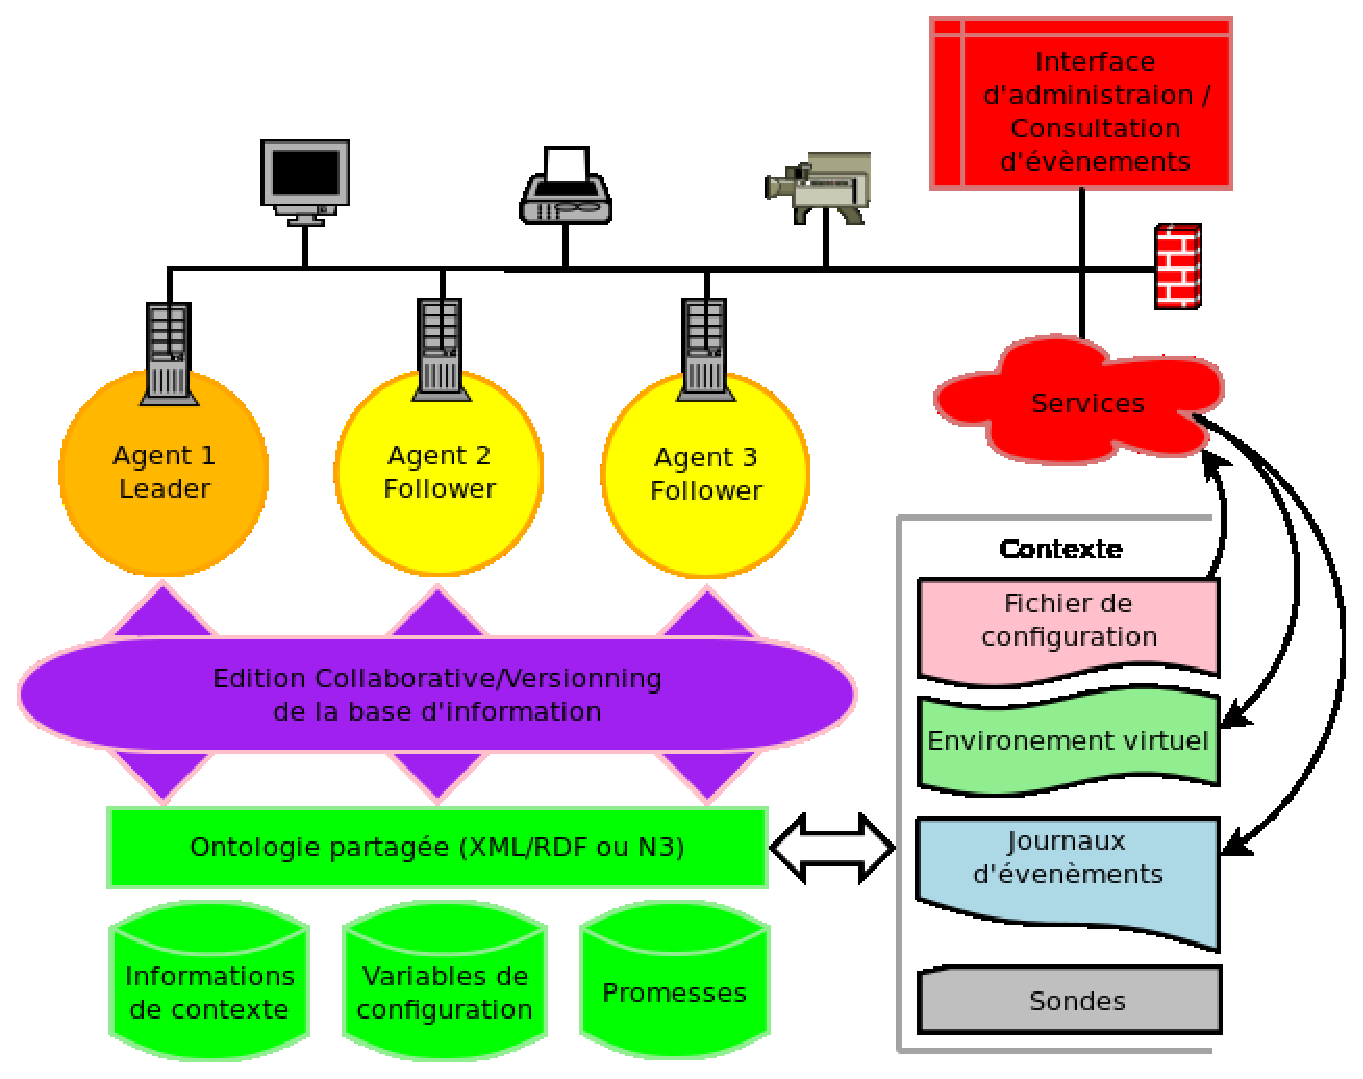
\includegraphics[width=.67\textwidth]{img/archi}
    \caption{Schéma d'implémentation du système multi-agents}
    \label{fig:archi}
%\end{wrapfigure}
\end{figure}

\section{Gestionnaire de configuration basé sur la théorie de la promesse}

\subsection{Ontologie de contexte}

La structure de base de l'ontologie de contexte a été implémentée à l'aide du
logiciel libre \emph{Protégé}. Elle met a disposition une définition générique
des composants les plus standards d'un réseau d'application comme les interfaces,
les processus, les utilisateurs ou encore les fichiers et leurs permissions
associées. Le détail des entités de cette ontologie est donné dans la section
\ref{sec:ontology}. La structure n'est pas figée, elle apporte seulement la
pierre angulaire pour la définition de nouveaux concepts plus spécifiques. En
effet, la structure s'étend à mesure que des sondes sont ajoutées.  Celle-ci
formalise un certain nombre d'informations de manière individuelle et la
structure découle alors de la mise en corrélation de ces informations.

\subsection{Sondes de contexte}

\begin{figure}[h]
    \scriptsize
    \begin{myverbatim}[commandchars=\\\{\},codes={\catcode`$=3\catcode`_=8}]
\textbf{user1@server1\$} trifle console

store   = Store()  # 10598 statements
server1 = Server() # uuid: d7c38143d6ed41c8ad1f04c9601733d1)
server2 = Server() # uuid: 4a1950ded8c141dd91b695e6f6a09f07)

>>> store
<trifle.store.Store instance at 0x336acf8>
>>> len(store.graph)
10598
>>> store.snapshot()
2014-08-14 15:08:07 \textbf{INFO} Pulling from InterfacesSensor...
2014-08-14 15:08:07 \textbf{DEBUG} 36 informations sensored
2014-08-14 15:08:07 \textbf{INFO} Pulling from ProcessesSensor...
2014-08-14 15:08:08 \textbf{WARNING} NoSuchProcess: 24963
2014-08-14 15:08:08 \textbf{WARNING} NoSuchProcess: 24964
2014-08-14 15:08:08 \textbf{WARNING} NoSuchProcess: 25080
2014-08-14 15:08:08 \textbf{WARNING} NoSuchProcess: 25082
2014-08-14 15:08:08 \textbf{DEBUG} 1395 informations sensored
2014-08-14 15:08:09 \textbf{INFO} Pulling from UsersSensor...
2014-08-14 15:08:09 \textbf{DEBUG} 15 informations sensored
[...]
>>> len(store.graph)
14534
    \end{myverbatim}
  \caption{Capture et fusion des informations de contexte provenant des sondes}
  \label{fig:sensor}
\end{figure}

Afin de garantir la flexibilité et l'extensibilité de notre gestionnaire, les
sondes de contextes sont implémentées sous la forme d'un greffon. Une classe
\emph{BaseSensor} est mise à disposition à titre de manifeste pour la création
de nouvelles sondes. L'interface implémente la méthode \emph{pull()} permettant
la population de l'ontologie de contexte.

Le processus de fusion des information est assez simple dans l'implémentation
puisqu'elle prend avantage des méthodes de manipulation de graphes intégrées à
la librairie Python RDFlib. Il ne peut exister ni d'informations redondantes, ni
de relations dépourvues d'acteurs : l'information demeure consistante.

Chacune de ces sondes va permettre de recueillir les informations relatives au
contexte local, c.a.d, les informations liées à la machine sur laquelle opère
l'agent. Lors de l'incrémentation d'un terme dans le cycle de fonctionnement
normal basé sur le consensus de Raft, les informations recueillies par chacun
des agents seront misent en corrélation. La méthode \emph{snapshot()} autorise
par ailleurs le renouvellement complet de la base d'informations.  La figure
\ref{fig:sensor} montre (partiellement) le résultat de cette méthode.  Une
information correspond à un triplet $\langle a P b \rangle$, où $b$ est une
valeur de la propriété $P$ pour le sujet $a$. Ne vous laissez pas confondre par
la terminologie : une relation, un prédicat et une propriété sont trois termes
pour la même notion. La relation $\langle a P b \rangle$ utilise le prédicat
$P$, et exprime que le sujet $a$ a une valeur $b$ pour la propriété $P$.

\subsection{Système multi-agents}

\subsubsection{Consensus de Raft}

%\begin{wrapfigure}{r}{.5\textwidth}
\begin{figure}[h]
  %\scriptsize
  %\centering

  %\begin{minipage}{.6\textwidth}
  %\begin{frame}[t,fragile]
  %\defverbatim[colored]\mycode{
    \scriptsize
    \begin{myverbatim}[commandchars=\\\{\},codes={\catcode`$=3\catcode`_=8}]
\textbf{user1@server1\$} trifle console

store   = Store()  # 10598 statements
server1 = Server() # uuid: d7c38143d6ed41c8ad1f04c9601733d1)
server2 = Server() # uuid: 4a1950ded8c141dd91b695e6f6a09f07)

>>> server1, server2
(<Server(Thread-1, started daemon 140389140690688)>, 
 <Server(Thread-2, started daemon 140388924913408)>)
>>> server1.role, server2.role
('follower', 'leader')
>>> server1.call\_election()
>>> server1.role, server2.role
('leader', 'follower')
    \end{myverbatim}
  %}
  %\end{frame}
  %\end{minipage}
  \caption{Validation de l'implémentation du consensus de Raft}
  \label{fig:raft}
%\end{wrapfigure}
\end{figure}

Le mécanismes que décrit le consensus de Raft ont été implémentés en Python.
Dans notre implémentation, on suppose qu'il n'existe qu'un seul agent par
machine. Tout d'abord, parce qu'il n'y a que très peu d'intérêts à déployer
plusieurs instances sur la même machine, et ensuite, parce que cela facilite
grandement le processus de découverte de nouvelles ressources. En effet, le
service (l'agent) sera mis à disposition à travers un port de communication
TCP/UDP figé : 6182 (hormis le fait qu'il n'est actuellement utilisé par aucune
application courante, le choix de ce port est complètement arbitraire). Ainsi,
il sera beaucoup moins coûteux de balayer chacune des plages du réseau à la
recherche de nouveaux agents.

Dans la figure \ref{fig:raft}, le gestionnaire est lancé en mode console. Le
serveur 1 correspond au serveur local et le serveur 2 est un serveur distant. À
l'initialisation du programme, une campagne est lancée et l'un des deux serveur
est élu \emph{leader}. Le \emph{follower} (serveur 2) va supposer une
défaillance du leader (arrêt des pulsations) et donc renouveler la campagne à
laquelle il est \emph{candidat} (et même favori). À l'issue de cette seconde
élection, on remarque que c'est désormais le second serveur qui est à la tête du
système et les opérations ont repris leur cours normal.

\subsubsection{Consistance de l'ontologie}

\begin{figure}[h]
    \scriptsize
    \begin{myverbatim}[commandchars=\\\{\},codes={\catcode`$=3\catcode`_=8}]
\textbf{SELECT} ?MachineName ?UserName ?PID ?IPv4Address ?Port ?ServiceName ?Command ?Status
\textbf{WHERE} \{
    ?Process   a             t:Process .
    ?Process   t:ProcessID   ?PID .
    ?Process   t:launchedBy  ?User .
    ?Process   t:runsOn      ?Machine .
    ?Process   t:Command     ?Command .
    ?Process   t:Name        ?ProcessName .
    ?Process   t:Status      ?Status .
    ?User      t:Name        ?UserName .
    ?Machine   t:Name        ?MachineName .
    ?Service   t:startedBy   ?Process .
    ?Service   t:ServicePort ?Port .
    ?Service   t:Status      ?Status .
    ?Interface t:componentOf ?Machine .
    ?Location  a             ?IPAddress .
    ?Location  t:Type        "IPv4"^^xsd:string .
    ?Location  t:locates     ?Interface .
    ?Location  t:Address     ?IPv4Address .
\}
    \end{myverbatim}
    \caption{Exemple de requête permettant de vérifier la consistance de l'ontologie}
    \label{fig:sparql}
\end{figure}

Afin de valider la consistance de l'ontologie, le procédé consiste à vérifier
la bonne mise en correspondance d'une certaine quantité d'informations
provenant d'agents et de sondes différentes. La figure \ref{fig:sparql} est un
exemple pertinent de requête permettant de justifier la bonne mise en
corrélation des informations de contexte. Cet requête permet d'obtenir la liste
détaillée de tous les services disponibles dans l'infrastructure, leurs hôtes
respectifs, ainsi que les processus auxquels ils sont attachés, la commande qui a
permit leur démarrage et même l'utilisateur propriétaire du processus. Cet
exemple invoque de multiples sondes dans le réseau. La sonde \emph{base}
permettant l'identification de la machine sur laquelle opère
l'agent. La sonde \emph{interfaces} permet d'associer des données d'adressage à
la machine courante. La sonde \emph{services} permet de détecter les différents
services dans le réseau et les ports sur lesquels ils sont distribués. La sonde
\emph{processus} autorise la lecture des états des différents processus. Enfin
la sonde \emph{user} permet le référencement des groupes et utilisateurs dans le
cluster.

\subsection{Interface d'administration}

Le gestionnaire de configuration prévoit une interface d'administration
pour la définition des politiques de comportement et le contrôle des différents
composants du système. L'interface est un service web distribué par
chacun des agents. Toutes les actions effectuées à travers l'interface seront
opérées par le leader du cluster afin de prévenir les problèmes liés à des
modifications concurrentes. L'ontologie de contexte sera directement
consultable en temps réel à l'aide de requêtes SPARQL. Enfin, elle doit
conserver la possibilité de renseigner les valeurs des variables de
configuration de bas niveau. Des captures d'écran de l'interface
d'administration sont disponibles en annexe \ref{appendix:interface}.

\section{Évaluation de la solution proposée}

\subsection{Limites de la solution}

%\begin{wrapfigure}{r}{.7\textwidth}
\begin{figure}[H]
    \centering
    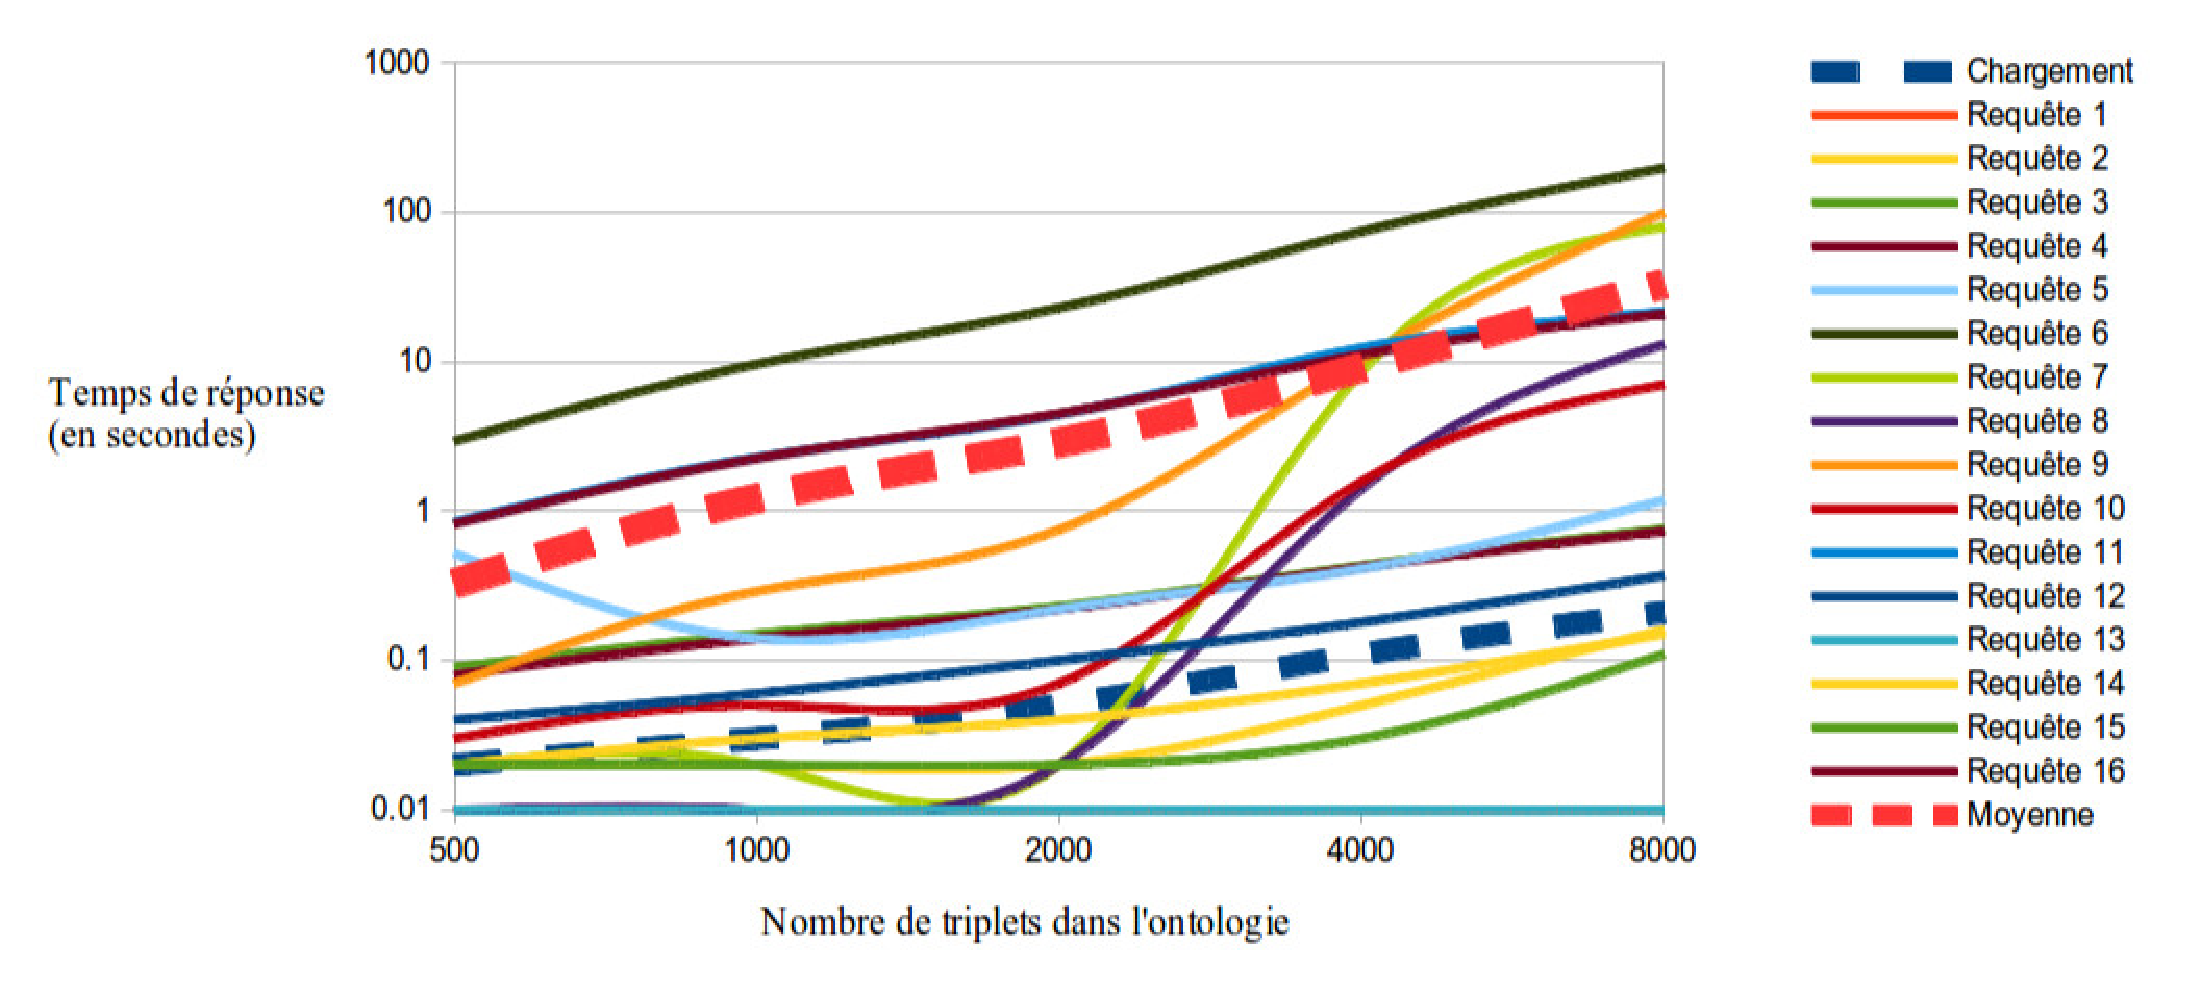
\includegraphics[width=\textwidth]{img/chart_sparql}
    \caption{Évaluation des performances de l'ontologie}
    \label{fig:chart}
%\end{wrapfigure}
\end{figure}

Dans cette étude, nous avons porté une attention accrue aux problématiques de
formalisation et de consistance de l'information. Le système actuel souffre
néanmoins de quelques lacunes en termes de performances. En effet, nous
remarquons que le temps de consultation de l'ontologie est étroitement lié à
la taille de cette dernière. La figure \ref{fig:chart} met bien en évidence ce
phénomène ; en mettant sur une échelle logarithmique les résultats des tests de
performances composés de 16 requêtes variées. On remarque que la ligne
rouge pointillée représentant la moyenne est droite, autrement dit, le temps de
consultation de l'ontologie est exponentiel vis-à-vis de sa taille.

\subsection{Perspectives d'évolution}

Dans cette implémentation, nous avons complètement laissé de coté tous les
aspects liés aux performances. Le prototype en l'état mériterait toutefois
quelques optimisations. La base d'échange (ontologie/journaux) est actuellement
gérée à l'aide des fichiers ; sa mise en tampon ou en base permettrait sans
aucuns doutes un accès beaucoup plus rapide.

Les sondes sont implémentées de manière à modéliser un maximum d'informations
et trouver les corrélations entre les différentes informations sondées. Elles
ne sont cependant pas interdépendantes d'un point de vue fonctionnel. Nous
pourrions par conséquent facilement paralléliser tout le processus de sondage.

Pour finir, l'ontologie de contexte implémentée pour cette preuve de concept
est très générique et entièrement ciblée sur l'environnement virtuel. Il semble
primordial d'apporter les outils et la documentation nécessaires pour permettre
à la communauté du libre de contribuer à la base de connaissance.

\section{Conclusion}

Les technologies basées sur le contexte vont jouer un rôle fondamental dans la
prochaine génération de systèmes informatiques à mesure que la complexité des
logiciels, la diversité et l'omniprésence des périphériques continuent
d'augmenter. Cependant, elle doivent offrir des mécanismes permettant la
gestion automatique des dépendances inter-composants et composant/ressource.
Dans le cas contraire, le développement de systèmes basés sur les composants
demeurera difficile à appréhender et conduira bien souvent à des systèmes peu
fiables et pas assez robustes.

Les environnements qui composeront l'informatique ubiquitaire de demain seront
composés de milliers de périphériques, avec des millions de composantes
logicielles. Les systèmes actuels s'appuient fortement sur la configuration
manuelle, ce qui à une telle échelle n'est plus gérable. Il n'existe que deux
issues possibles à cette situation : une configuration statique, ou une
configuration dynamique et automatique. Puisque les environnements ont
tendance à être de plus en plus dynamiques, la configuration autonome semble
incarner la seule solution viable.

% ex: set spelllang=fr spell: %
%%% Local Variables: ***
%%% mode: latex ***
%%% TeX-master: "thesis.tex" ***
%%% End: ***
